\documentclass[justified]{tufte-handout}
\usepackage{microtype}
\usepackage{amsmath}
\usepackage{graphicx}
\title{Second Order High Pass Filter}
\author{Chris Curro}
\date{\today}
\setlength{\textheight}{650pt}
\begin{document}
\maketitle
\begin{abstract}
As per the project specification, a second order high pass filter was
constructed with a Sallen-Key topology. The corner frequency for this filter is
about 100~Hz.
\end{abstract}
\section{Design}
\vspace{-0.2in}
\begin{figure}[h]
\centering
\label{schemSim}
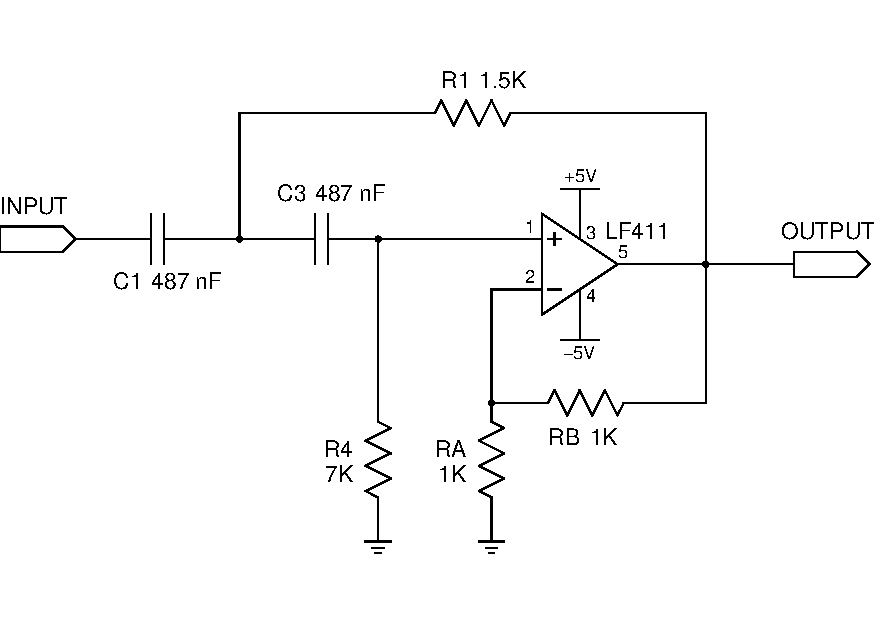
\includegraphics[width=0.9\linewidth,trim=0 .3in 0 .35in,clip=true]{schemSim.pdf}
\caption{Proposed schematic for the filter.}
\end{figure}
\paragraph{} The first step in the design process was selecting the appropriate
components to meet the specification. The specification was a Butterworth filter with a cuttoff frequency of 100~Hz. Furthermore two
constraints were set which reduced the size of the parameter space; the two
capacitors were constrained to be of equal value and the DC voltage gain of the
system was set to be 2 (6~dB). The latter constraint imposes the condition that
$R_A = R_B$ by the equation:
\begin{equation}
K = 1 + \frac{R_B}{R_A}
\end{equation}
Combining the constraints and acknowledging the fact that this circuit is
Butterworth filter the following equation can be written for the Q-Factor:
\begin{equation}
\frac{1}{Q} = \sqrt{2} = (1-K)\sqrt{\frac{R_4}{R_2}} + 2\sqrt{\frac{R_2}{R_4}}
\end{equation}
Solving this equation, a final constraint becomes evident:
\begin{equation}
R_4 = R_2(3+\sqrt{5})
\end{equation}
% Taking this into consideration a value of 1 k$\Omega$ was selected for $R_1$;
% therefore $R_2$ is required to be 2 k$\Omega$. These values were selected
% because 1 k$\Omega \pm 1\%$ resistors were available in the lab, therefore it
% was easier to meet the correct ratio. Additionally for this $R_A$ and $R_B$ were
% set to be 1~k$\Omega$ as well.
\paragraph{} The last remaining parameters were $C_1$ and $C_3$ which were
already constrained to be equal to each other (denoted as $C$). Incorporating
this constraint and the Sallen-Key topology, the parameter can be solved for
with the following equation:
\begin{equation}
2\pi f_c = \frac{1}{\sqrt{R_2R_4C^2}}
\end{equation}
This equation can rewrittern to give an expression for $C$ in terms of $R_2$
$R_4$. Using the ratio of $R_2$ and $R_4$ above, this expression can be
simplified to use only $R_2$. Using this expression, a linear sweep was
performed to find a value for $R_2$ that resulting an a $C$ value that was
available in the lab. This theorecal value was 460~nF. Ultimately the
capacitors used had a value of 487~nF as measured by a RSR M9803R
Multimeter. 

Using the measured values for the matched capacitors, new values were calculated
for $R_2$ and $R_4$. In order to hit the corner frequency correctly while
maintaining reasonable resistor values the precise ratio for $R_2$ and $R_4$ was
broken. The new values for $R_2$ and $R_4$ were 1.5 k$\Omega$ and $7$ k$\Omega$
respectively. These values were achieved precisely with parallel/series
combinations of 1 k$\Omega \pm 1\%$ resistors. While the $Q$ was off of the
correct value for a Butterworth filter, simulation confirmed that the behavior
would still agree with a Butterworth response.
\begin{figure}
\centering
\label{simRes}
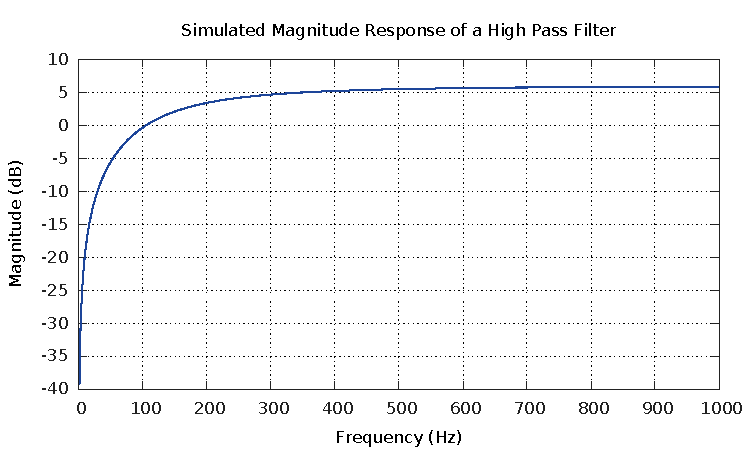
\includegraphics[width=0.9\linewidth]{simResponse.pdf}
\caption{Simulated frequency response of the high pass filter}
\end{figure}
When constructed, the experimental results did match the simulation. In fact the
circuit was unstable, randomly throwing rail voltages at the output. Various
attempts at debugging were made, but ultimately the only way the circuit would
give a stable response was if the gain of two was forfeited and instead had
unity gain. By changing the gain the Q factor was adjusted even further, so the
filter did not give the planned Butterworth response, but instead gave a
Chebyshev Type 1 response, with a a very weak, long ripple in the passband.
\begin{marginfigure}
\centering
\label{schemExp}
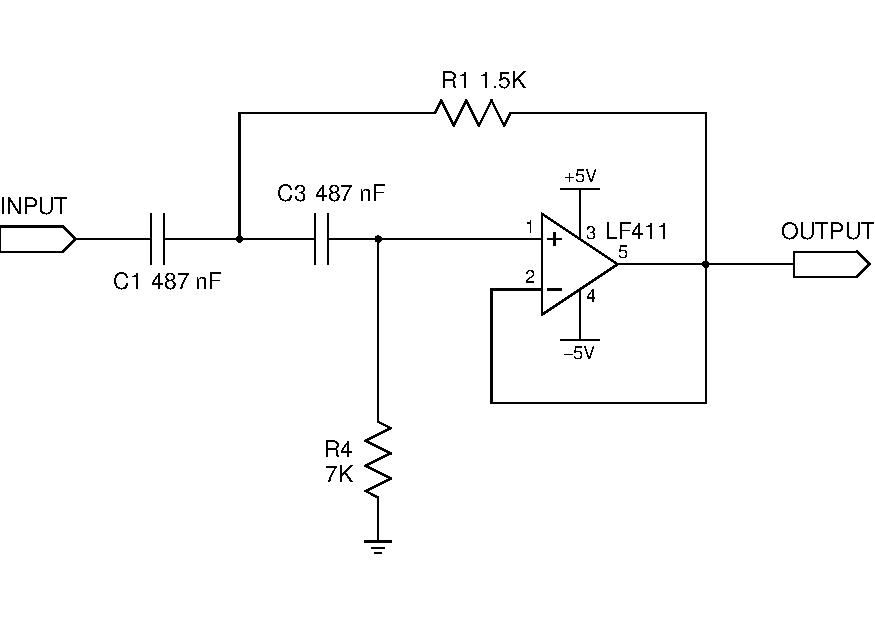
\includegraphics[width=1.1\linewidth,trim=0 .3in 0 .35in,clip=true]
{schemExp.pdf}
\caption{Final schematic for the filter.}
\end{marginfigure}
\clearpage
\section{Test Procedure and Results}
\paragraph{Frequency Response} The magnitude frequency response was
measured with a Hewlett Packard 35660A Dynamic Signal Analyzer from 10~Hz up to
1000~Hz. These results are summarized in Figure \ref{expRes}. Measurements were
made every 5~Hz up to 100~Hz, then every 10~Hz up to 200~Hz, and then every
100~Hz for the remainder of the span. The HP 35660A was responsible for both
stimulating the device under test and measuring the response.
\begin{figure}
\centering
\label{expRes}
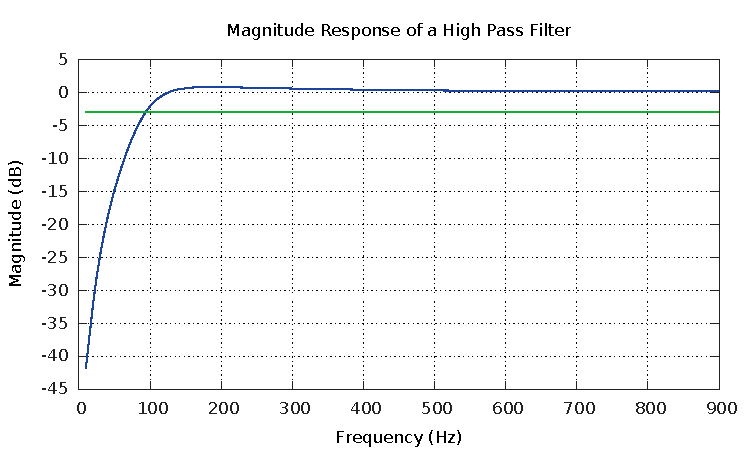
\includegraphics[width=0.9\linewidth]{expResponse.pdf}
\caption{Experimental frequency response of the high pass filter}
\end{figure}
\paragraph{Power Consumption}
In order to measure the power consumption for a 100 Hz input signal, the 
voltage and current readouts on the power supply unit (a Gwinstek GPS-3303) were
recorded. From these (probably ridiculously inaccurate) measurements, the power
consumption is approximately 200 mW.
\end{document}